\documentclass{beamer}
\usepackage[utf8]{inputenc}
\usepackage{graphicx}

% --- Tema y colores ---
\usetheme{Madrid}
\usecolortheme{beaver}

% --- Información del Título ---
\title{QUCS-S: Tu Laboratorio Electrónico Virtual}
\author{Flores Oropeza Osvaldo}
\institute{UPIITA - IPN}
\date{\today}

\begin{document}

% --- Diapositiva del Título ---
\begin{frame}
  \titlepage
\end{frame}

% --- Diapositiva de Introducción ---
\begin{frame}{¿Qué es QUCS-S?}
  \begin{columns}
    \begin{column}{0.6\textwidth}
      \begin{itemize}
        \item Es un \textbf{simulador de circuitos electrónicos} de código abierto.
        \pause
        \item ¡Imagina un laboratorio virtual en tu computadora donde puedes diseñar y probar circuitos sin riesgo!
        \pause
        \item La "S" en su nombre viene de su integración con \textbf{SPICE}, un motor de simulación estándar en la industria.
        \pause
        \item Te permite dibujar esquemáticos, simularlos y visualizar los resultados.
      \end{itemize}
    \end{column}
    \begin{column}{0.4\textwidth}
        % Puedes agregar un logo o imagen aquí si quieres
        % \includegraphics[width=\textwidth]{logo_qucs.png}
        \centering
        \Huge \textbf{QUCS-S}
    \end{column}
  \end{columns}
\end{frame}

% --- Diapositiva de Utilidad ---
\begin{frame}{¿Para qué nos ayuda?}
  Es una herramienta fundamental para:
  \begin{itemize}
    \item \textbf{Aprender Electrónica:} Experimenta sin miedo a dañar componentes físicos. ¡Es la mejor forma de ver la teoría en acción!
    \pause
    \item \textbf{Verificar Diseños:} Antes de soldar, puedes asegurarte de que tu idea funciona correctamente.
    \pause
    \item \textbf{Realizar Mediciones Virtuales:} Usa instrumentos como osciloscopios, multímetros y analizadores para medir voltaje, corriente y otras señales en cualquier parte de tu circuito.
    \pause
    \item \textbf{Analizar el Comportamiento:} Entiende cómo responde tu circuito a diferentes condiciones (DC, AC, transitorio, etc.).
  \end{itemize}
\end{frame}

% --- Diapositiva de Alternativas ---
\begin{frame}{¿Qué programas puede sustituir?}
  QUCS-S es una alternativa \textbf{gratuita y de código abierto} a software comercial muy popular en la industria:
  \begin{columns}
    \begin{column}{0.5\textwidth}
      \begin{center}
        \textbf{Alternativas Comerciales}
        \begin{itemize}
          \item Multisim
          \item Proteus
          \item OrCAD
        \end{itemize}
      \end{center}
    \end{column}
    \begin{column}{0.5\textwidth}
      \begin{center}
        \textbf{Ventaja de QUCS-S}
        \begin{itemize}
          \item Sin costo de licencia.
          \item Acceso al código fuente.
          \item Multiplataforma (Windows, Linux, macOS).
        \end{itemize}
      \end{center}
    \end{column}
  \end{columns}
\end{frame}

% --- Diapositiva de Instalación con ESPACIO PARA IMÁGENES ---
\begin{frame}[fragile]{Instalación en Ubuntu: Paso a Paso}

  % --- Columna para el Primer Paso ---
  \begin{columns}[T] % La opción [T] alinea las columnas por la parte superior
    
    % Columna izquierda para el texto
    \begin{column}{0.5\textwidth}
      \begin{enumerate}
        \item \textbf{Verificar tu versión de Ubuntu}
          \begin{itemize}
            \item Abre la terminal (\texttt{Ctrl+Alt+T}) y escribe:
            \item \texttt{lsb\_release -a}
          \end{itemize}
      \end{enumerate}
    \end{column}

    % Columna derecha para la imagen
    \begin{column}{0.5\textwidth}
      % --- AQUÍ VA TU IMAGEN ---
      % Reemplaza "paso1-version.png" con el nombre de tu archivo
      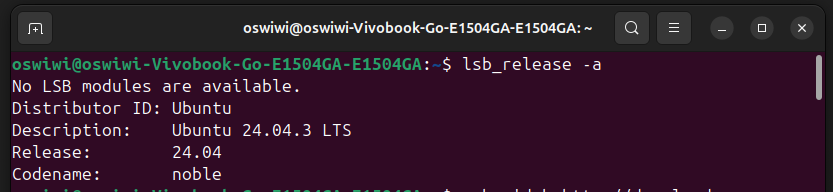
\includegraphics[width=\columnwidth]{Imagenes/InsP1.png}
    \end{column}

  \end{columns}
\end{frame}

\begin{frame}[fragile]{Instalación en Ubuntu: Paso 2}
  \framesubtitle{Añadir el Repositorio del Software}

  \begin{columns}[T]
    % Columna izquierda para el texto
    \begin{column}{0.5\textwidth}
      \begin{enumerate}
        \setcounter{enumi}{1} % Continuar la numeración desde el 2
        \item \textbf{Añadir el repositorio}
          \begin{itemize}
            \item Este comando le dice a tu sistema dónde buscar los paquetes de QUCS-S.
            \item \small{\texttt{echo 'deb ...' | sudo tee /etc/apt/...}}
          \end{itemize}
      \end{enumerate}
    \end{column}

    % Columna derecha para la imagen
    \begin{column}{0.5\textwidth}
      % Reemplaza "paso2-repo.png" con el nombre de tu archivo
      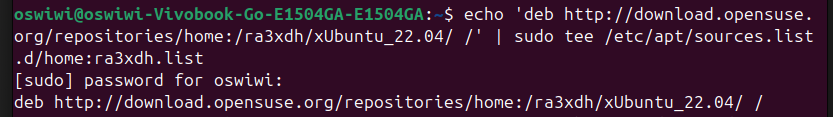
\includegraphics[width=\columnwidth]{Imagenes/InsP2.png}
    \end{column}
  \end{columns}
\end{frame}

\begin{frame}[fragile]{Instalación en Ubuntu: Paso 3}
  \framesubtitle{Importar la Clave de Seguridad}

  \begin{columns}[T]
    % Columna izquierda para el texto
    \begin{column}{0.5\textwidth}
      \begin{enumerate}
        \setcounter{enumi}{2} % Continuar la numeración desde el 3
        \item \textbf{Importar la clave GPG}
          \begin{itemize}
            \item Esto es como una firma digital. Le asegura a tu sistema que el software que descargas es auténtico y seguro.
            \item \small{\texttt{curl -fsSL ... | gpg --dearmor | sudo tee ...}}
          \end{itemize}
      \end{enumerate}
    \end{column}

    % Columna derecha para la imagen
    \begin{column}{0.5\textwidth}
      % Reemplaza "paso3-key.png" con el nombre de tu archivo
      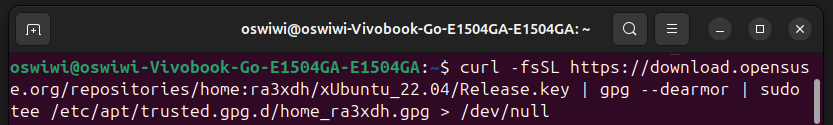
\includegraphics[width=\columnwidth]{Imagenes/InsP3.png}
    \end{column}
  \end{columns}
\end{frame}

\begin{frame}[fragile]{Instalación en Ubuntu: Paso 4}
  \framesubtitle{Actualizar y ¡A Instalar!}

  \begin{columns}[T]
    % Columna izquierda para el texto
    \begin{column}{0.5\textwidth}
      \begin{enumerate}
        \setcounter{enumi}{3} % Continuar la numeración desde el 4
        \item \textbf{Actualizar e Instalar}
          \begin{itemize}
            \item \texttt{sudo apt update}: Actualiza la lista de software disponible.
            \item \texttt{sudo apt install qucs-s}: ¡Descarga e instala el programa!
          \end{itemize}
      \end{enumerate}
    \end{column}

    % Columna derecha para la imagen
    \begin{column}{0.5\textwidth}
      % --- PRIMERA CAPTURA ---
      % Reemplaza con el nombre de tu captura del "update"
      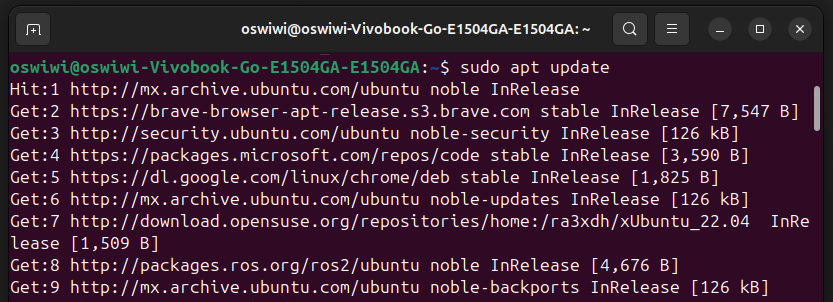
\includegraphics[width=\columnwidth]{Imagenes/InsP4-1.png}
      
      \vspace{0.3cm} % Espacio vertical entre las dos imágenes
      
      % --- SEGUNDA CAPTURA ---
      % Reemplaza con el nombre de tu captura del "install"
      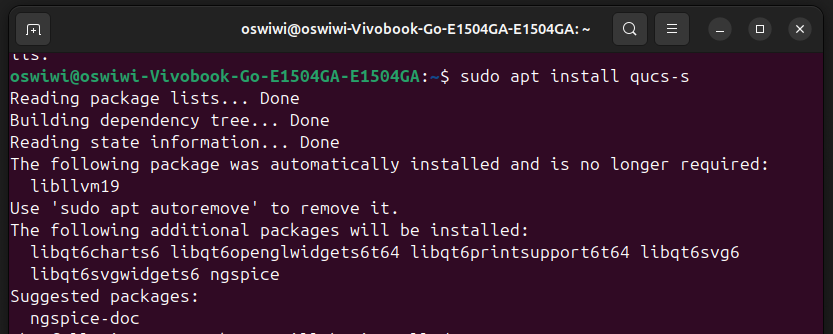
\includegraphics[width=\columnwidth]{Imagenes/InsP4-2.png}
    \end{column}
  \end{columns}
\end{frame}

\begin{frame}[fragile]{Instalación en Windows (¡Muy Fácil!)}

  \begin{columns}[T] % Alinea las columnas por la parte superior
    
    % --- Columna Izquierda: Las Instrucciones ---
    \begin{column}{0.5\textwidth}
      
      % El bloque del Paso 1 aparece en el slide 1 y se queda
      \begin{block}<1->{Paso 1: Descargar el Instalador}
        Primero, ve a la página oficial de descargas de QUCS y busca el archivo comprimido de nombre \textbf{qucs-0.0.19-win32...adms.zip}.
        \vspace{0.2cm}
        
        \tiny{\texttt{https://sourceforge.net/projects/qucs/files /qucs-binary/0.0.19/}}
      \end{block}
      
      % El bloque del Paso 2 solo aparece a partir del slide 2
      \begin{block}<2->{Paso 2: Ejecutar el Programa}
        \begin{itemize}
          \item Una vez descargado, extrae la el archivo \texttt{.zip}.
          \item Abre la carpeta y busca el archivo \texttt{qucs}.
          \item ¡Solo tienes que dar doble clic y empezar a trabajar!
        \end{itemize}
      \end{block}
      
    \end{column}
    
    % --- Columna Derecha: Las Capturas de Pantalla ---
    \begin{column}{0.5\textwidth}
      
      % La imagen del Paso 1 aparece en el slide 1 y se queda
      \includegraphics<1->[width=\columnwidth]{Imagenes/InsWinP1.png}
      
      % La imagen del Paso 2 (y su espacio) solo aparecen a partir del slide 2
      \only<2->{
        \vspace{0.3cm} % Espacio entre imágenes
        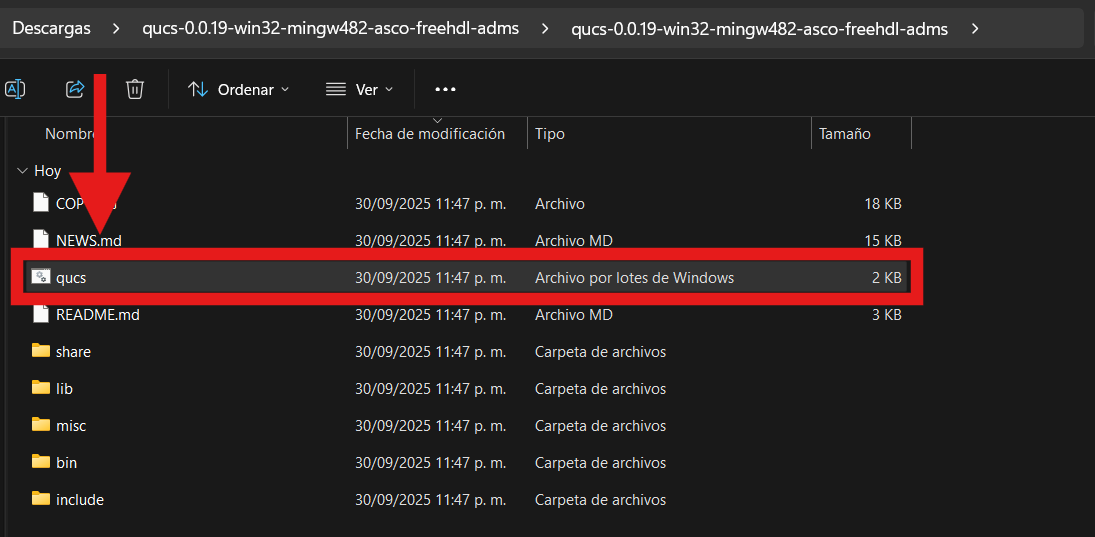
\includegraphics[width=\columnwidth]{Imagenes/InsWinP2.png}
      }
      
    \end{column}
    
  \end{columns}
\end{frame}

% --- Diapositiva de Ejemplo ---
\begin{frame}[fragile]{Ejemplo: Iniciando en el entorno QUCS-S}

  % --- Espacio de trabajo ---
  \begin{columns}[T] % La opción [T] alinea las columnas por la parte superior
    
    % Columna izquierda para el texto
    \begin{column}{0.5\textwidth}
      \begin{enumerate}
        \item \textbf{Espacio de Trabajo}
          \begin{itemize}
            \item Barra de tareas (\textit{Rojo}).
            \item Barra de componentes (\textit{Verde}).
            \item Hoja de trabajo (\textit{Azul}).
          \end{itemize}
      \end{enumerate}
    \end{column}

    % Columna derecha para la imagen
    \begin{column}{0.5\textwidth}
      % --- AQUÍ VA TU IMAGEN ---
      % Reemplaza "paso1-version.png" con el nombre de tu archivo
      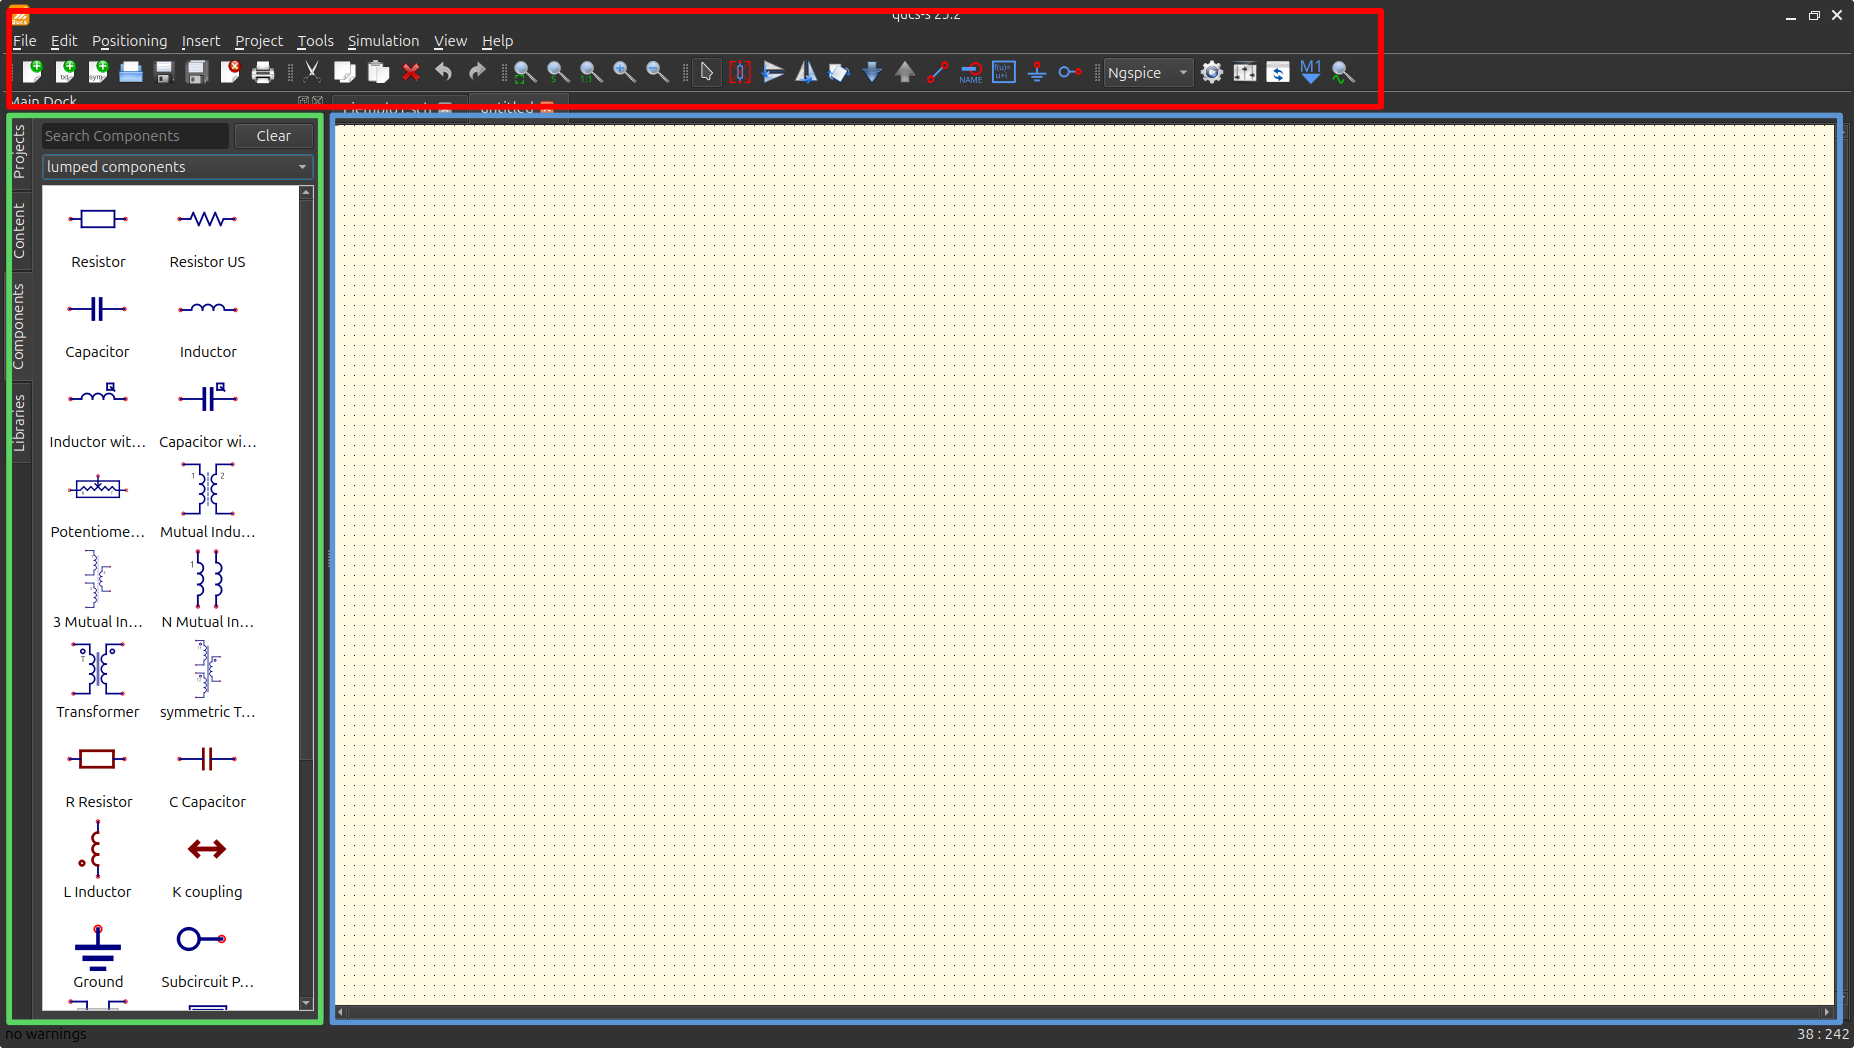
\includegraphics[width=\columnwidth]{Imagenes/ToolB.png}
    \end{column}

  \end{columns}
\end{frame}

\begin{frame}[fragile]{Ejemplo: Iniciando en el entorno QUCS-S}
  \framesubtitle{Inclusión y modificación de componentes}

  \begin{columns}[T]
    % Columna izquierda para el texto
    \begin{column}{0.5\textwidth}
      \begin{enumerate}
        \setcounter{enumi}{1} % Continuar la numeración desde el 2
        \item \textbf{Componentes}
          \begin{itemize}
            \item Seleccionar y arrastrar a la hoja de trabajo.
            \item Clic derecho $->$ Editar propiedades.
          \end{itemize}
      \end{enumerate}
    \end{column}

    % Columna derecha para la imagen
    \begin{column}{0.5\textwidth}
      % Reemplaza "paso2-repo.png" con el nombre de tu archivo
      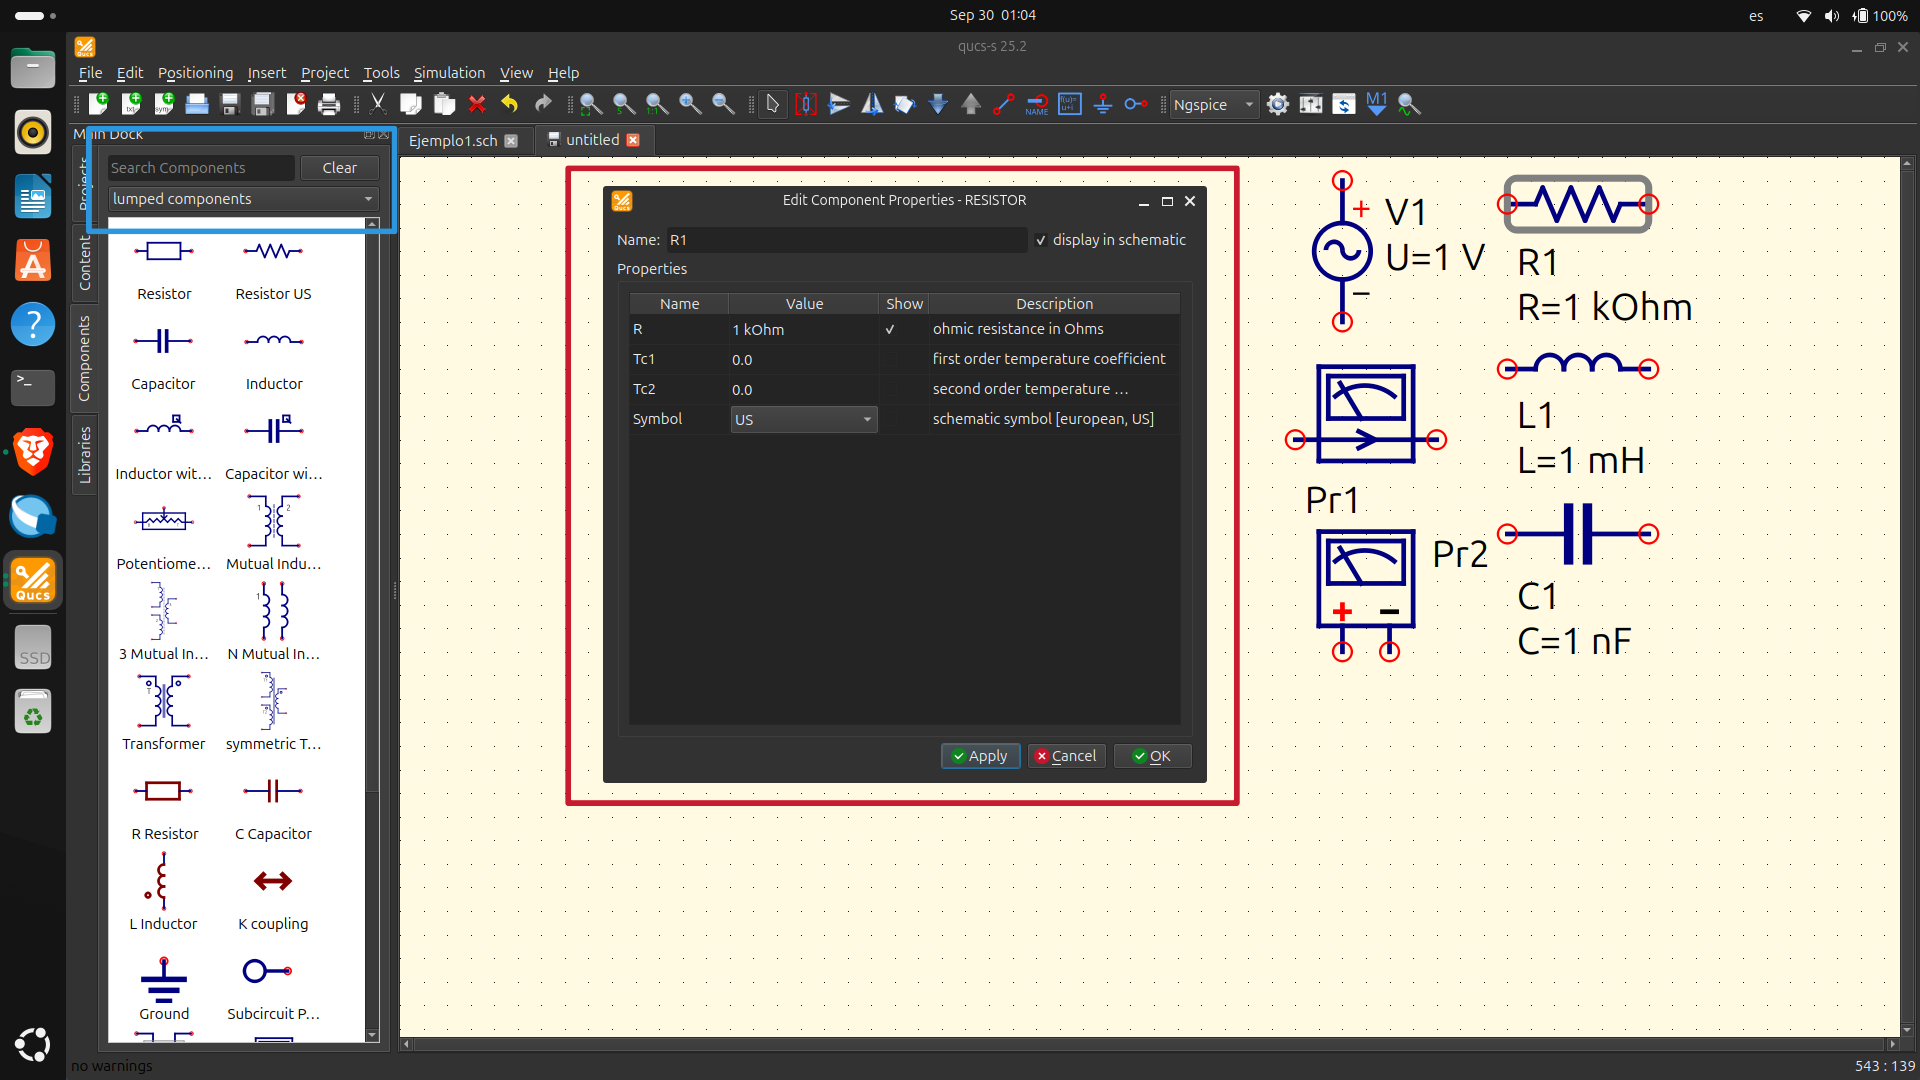
\includegraphics[width=\columnwidth]{Imagenes/Comps.png}
    \end{column}
  \end{columns}
\end{frame}

\begin{frame}[fragile]{Ejemplo: Iniciando en el entorno QUCS-S}
  \framesubtitle{Armando un circuito RCL}

  \begin{columns}[T]
    % Columna izquierda para el texto
    \begin{column}{0.5\textwidth}
      \begin{enumerate}
        \setcounter{enumi}{2} % Continuar la numeración desde el 3
        \item \textbf{Componentes de medición y simulación}
          \begin{itemize}
            \item En la barra de componentes seleccionamos el menú \textit{Probes} $->$ Sonda de tensión. 
            \item En la barra de componentes seleccionamos el menú \textit{Probes} $->$ Sonda de corriente. 
            \item En la barra de componentes seleccionamos el menú \textit{Simulations} $->$ Simulación transitoria. 
          \end{itemize}
      \end{enumerate}
    \end{column}

    % Columna derecha para la imagen
    \begin{column}{0.5\textwidth}
      % Reemplaza "paso3-key.png" con el nombre de tu archivo
      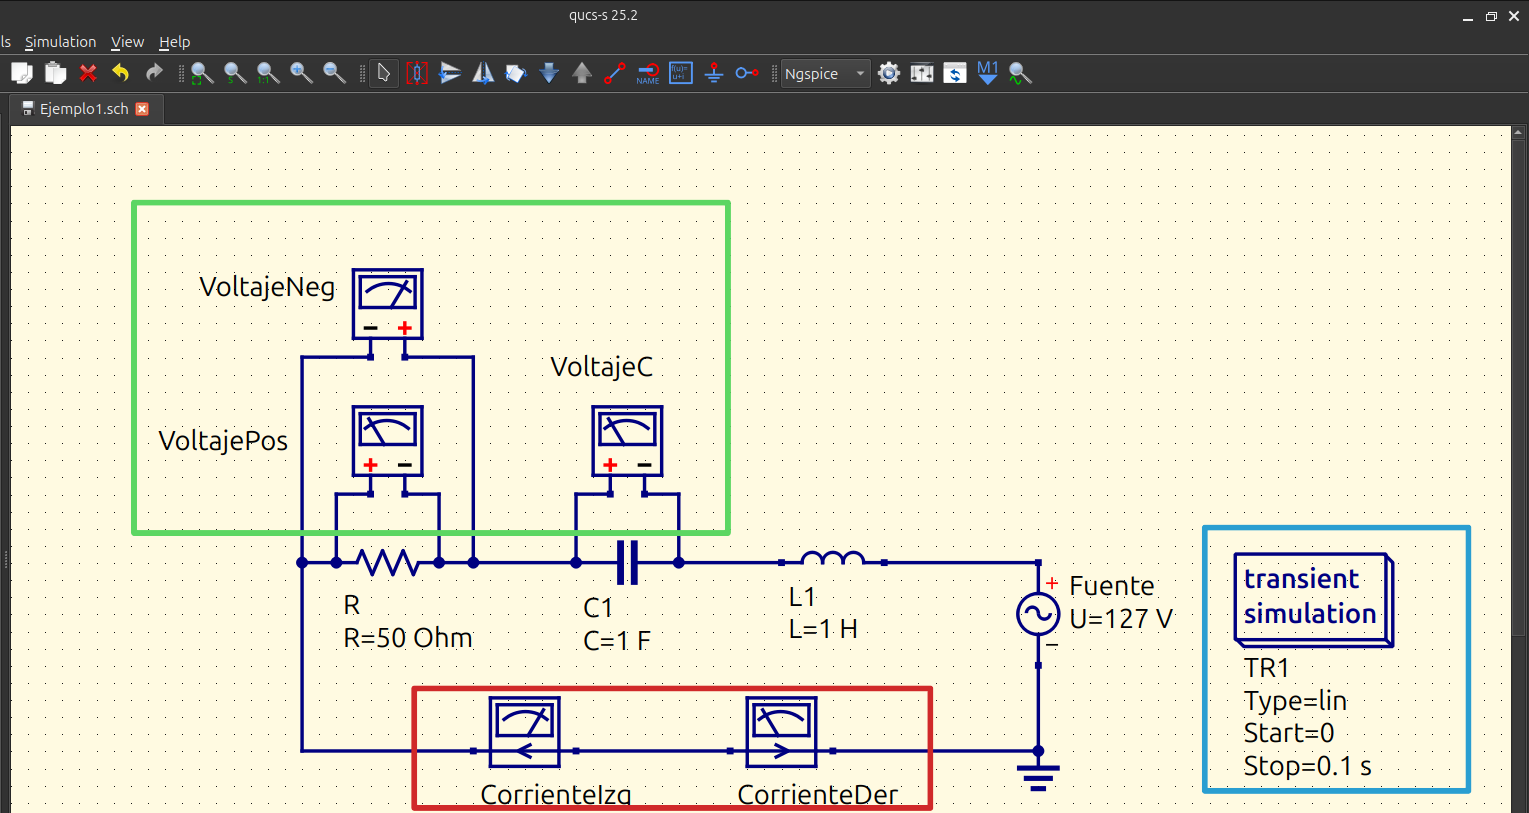
\includegraphics[width=\columnwidth]{Imagenes/Circ.png}
    \end{column}
  \end{columns}
\end{frame}

\begin{frame}[fragile]{Ejemplo: Iniciando en el entorno QUCS-S}
  \framesubtitle{¡A Simular!}

  \begin{columns}[T]
    % Columna izquierda para el texto
    \begin{column}{0.5\textwidth}
      \begin{enumerate}
        \setcounter{enumi}{3} % Continuar la numeración desde el 4
        \item \textbf{Simulación}
          \begin{itemize}
            \item \textbf{Primero}: Guardamos el archivo.
            \item \textbf{Segundo}: Seleccionamos el engrane (\textit{Simular}).
          \end{itemize}
      \end{enumerate}
    \end{column}

    % Columna derecha para la imagen
    \begin{column}{0.5\textwidth}
      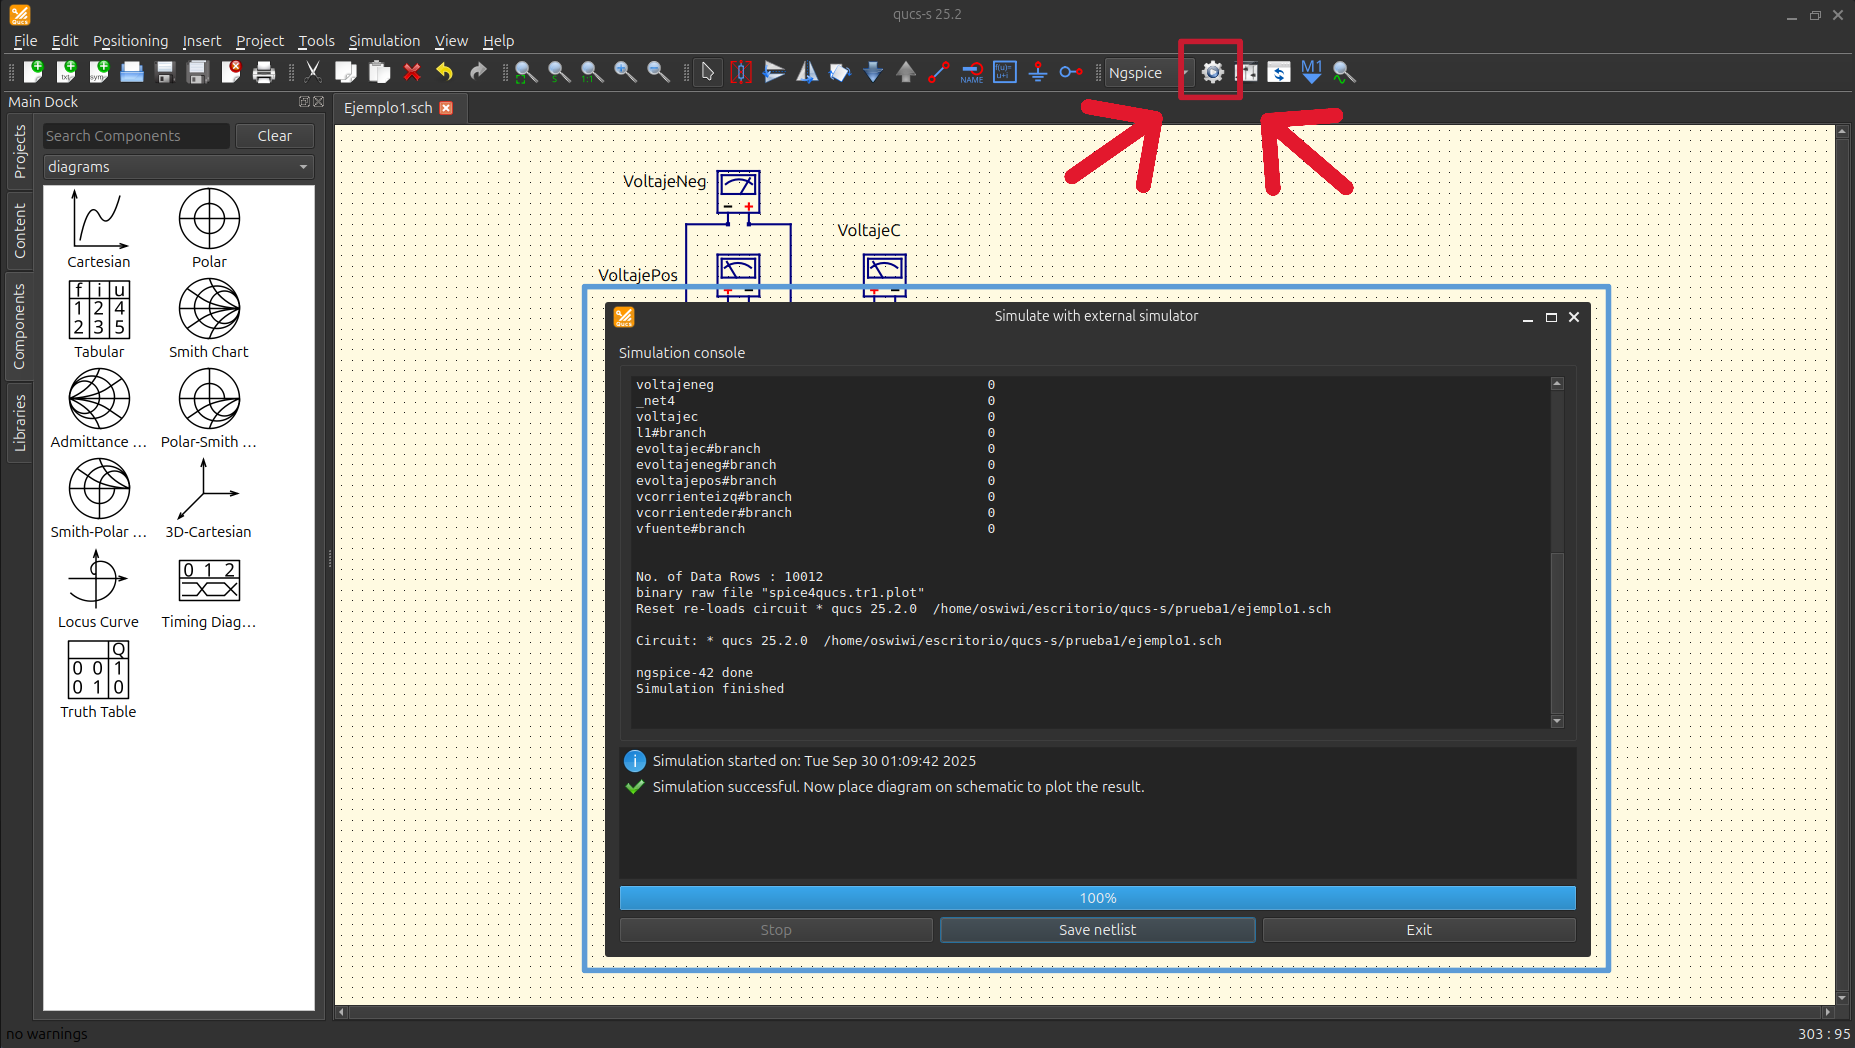
\includegraphics[width=\columnwidth]{Imagenes/Sim.png}
    \end{column}
  \end{columns}
\end{frame}

\begin{frame}[fragile]{Ejemplo: Iniciando en el entorno QUCS-S}
  \framesubtitle{Graficando los resultados}

  \begin{columns}[T]
    % Columna izquierda para el texto
    \begin{column}{0.5\textwidth}
      \begin{enumerate}
        \setcounter{enumi}{3} % Continuar la numeración desde el 4
        \item \textbf{Gráficas}
          \begin{itemize}
            \item Si salió bien la simulación aparecerá automáticamente el menú de diagramas.
            \item \textbf{Primero}: Seleccionamos diagrama \textit{Cartesiano}.
            \item \textbf{Segundo}: Doble clic sobre la medición que queremos graficar
            \item \textbf{Tercero}: Apply $->$ Ok.
          \end{itemize}
      \end{enumerate}
    \end{column}

    % Columna derecha para la imagen
    \begin{column}{0.5\textwidth}
      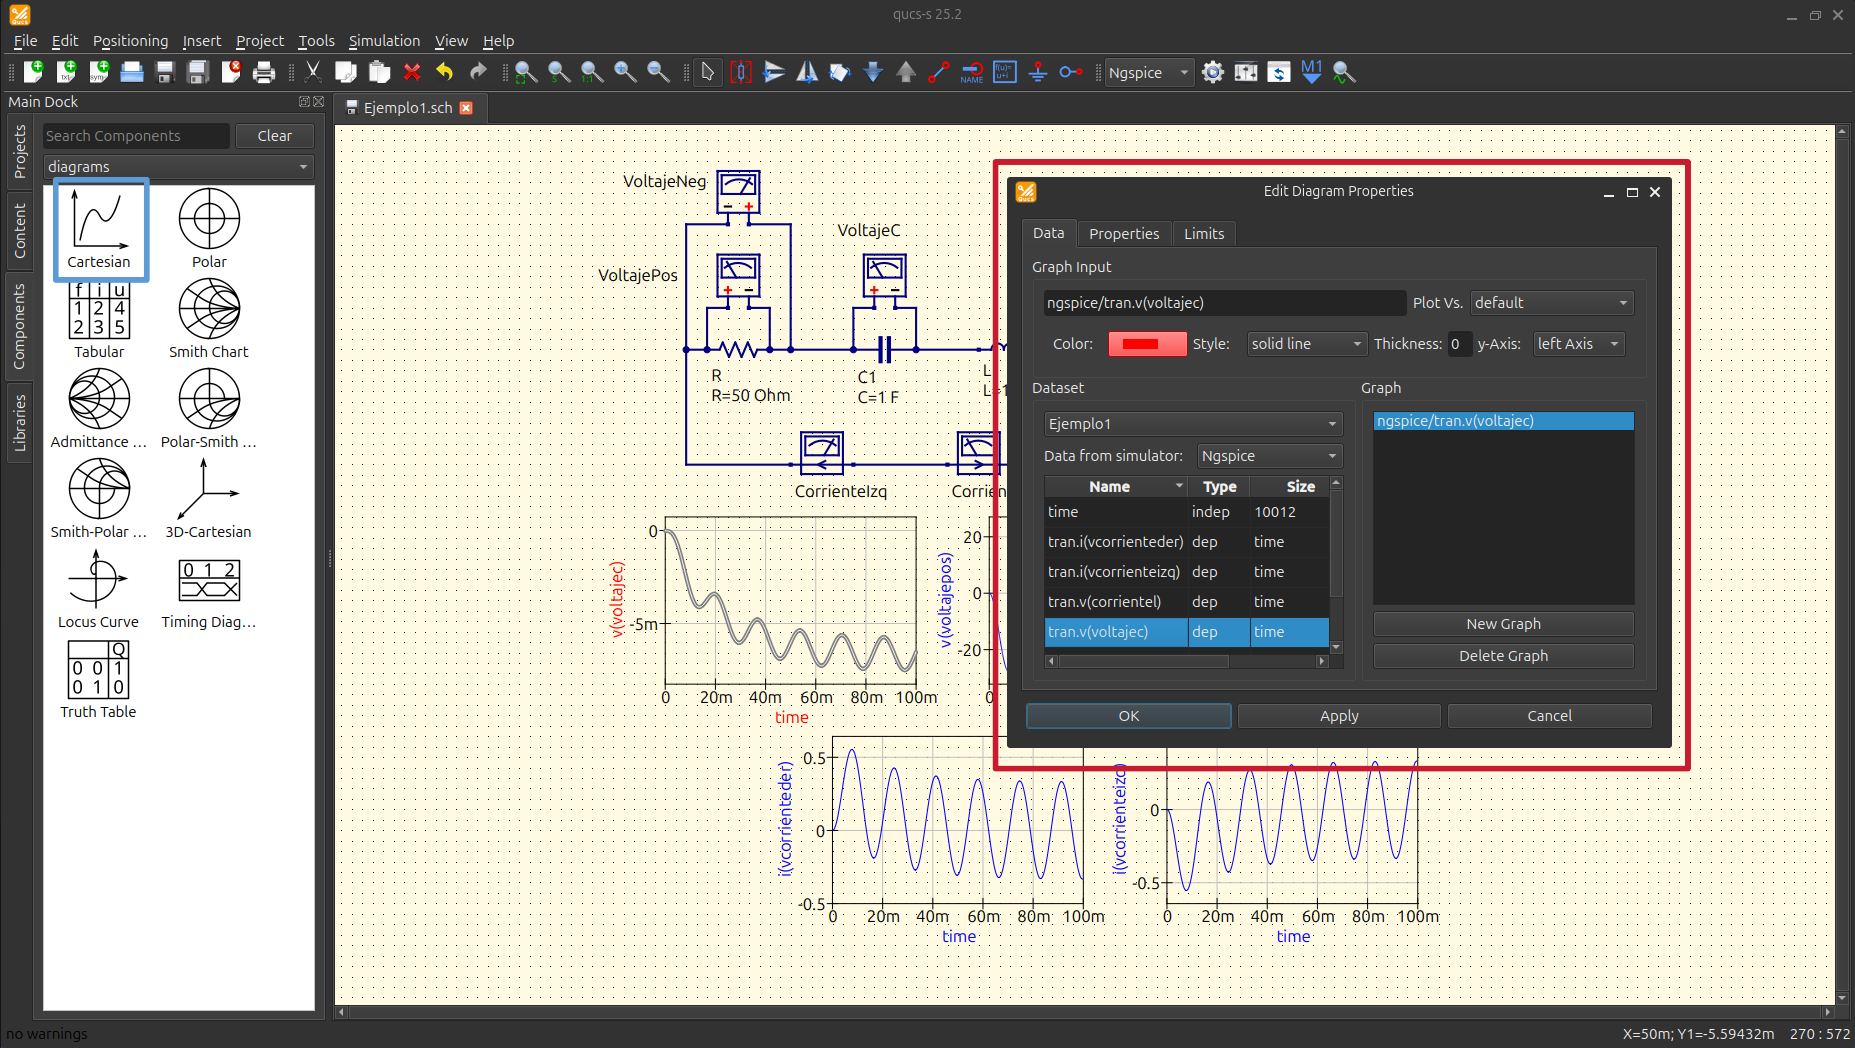
\includegraphics[width=\columnwidth]{Imagenes/Graph.png}
    \end{column}
  \end{columns}
\end{frame}

\begin{frame}[fragile]{Ejemplo: Iniciando en el entorno QUCS-S}
  \framesubtitle{¡Agrega los diagramas que quieras!}

  \begin{columns}[T]
    % Columna izquierda para el texto
    \begin{column}{0.5\textwidth}
      \begin{enumerate}
        \setcounter{enumi}{3} % Continuar la numeración desde el 4
        \item \textbf{Gráficas, tablas y más ...}
          \begin{itemize}
            \item QUCS-S contiene diferentes tipos de diagramas para las diferentes necesidades del usuario, desde gráficas y tablas de verdad hasta gráficas 3D.
          \end{itemize}
      \end{enumerate}
    \end{column}

    % Columna derecha para la imagen
    \begin{column}{0.5\textwidth}
      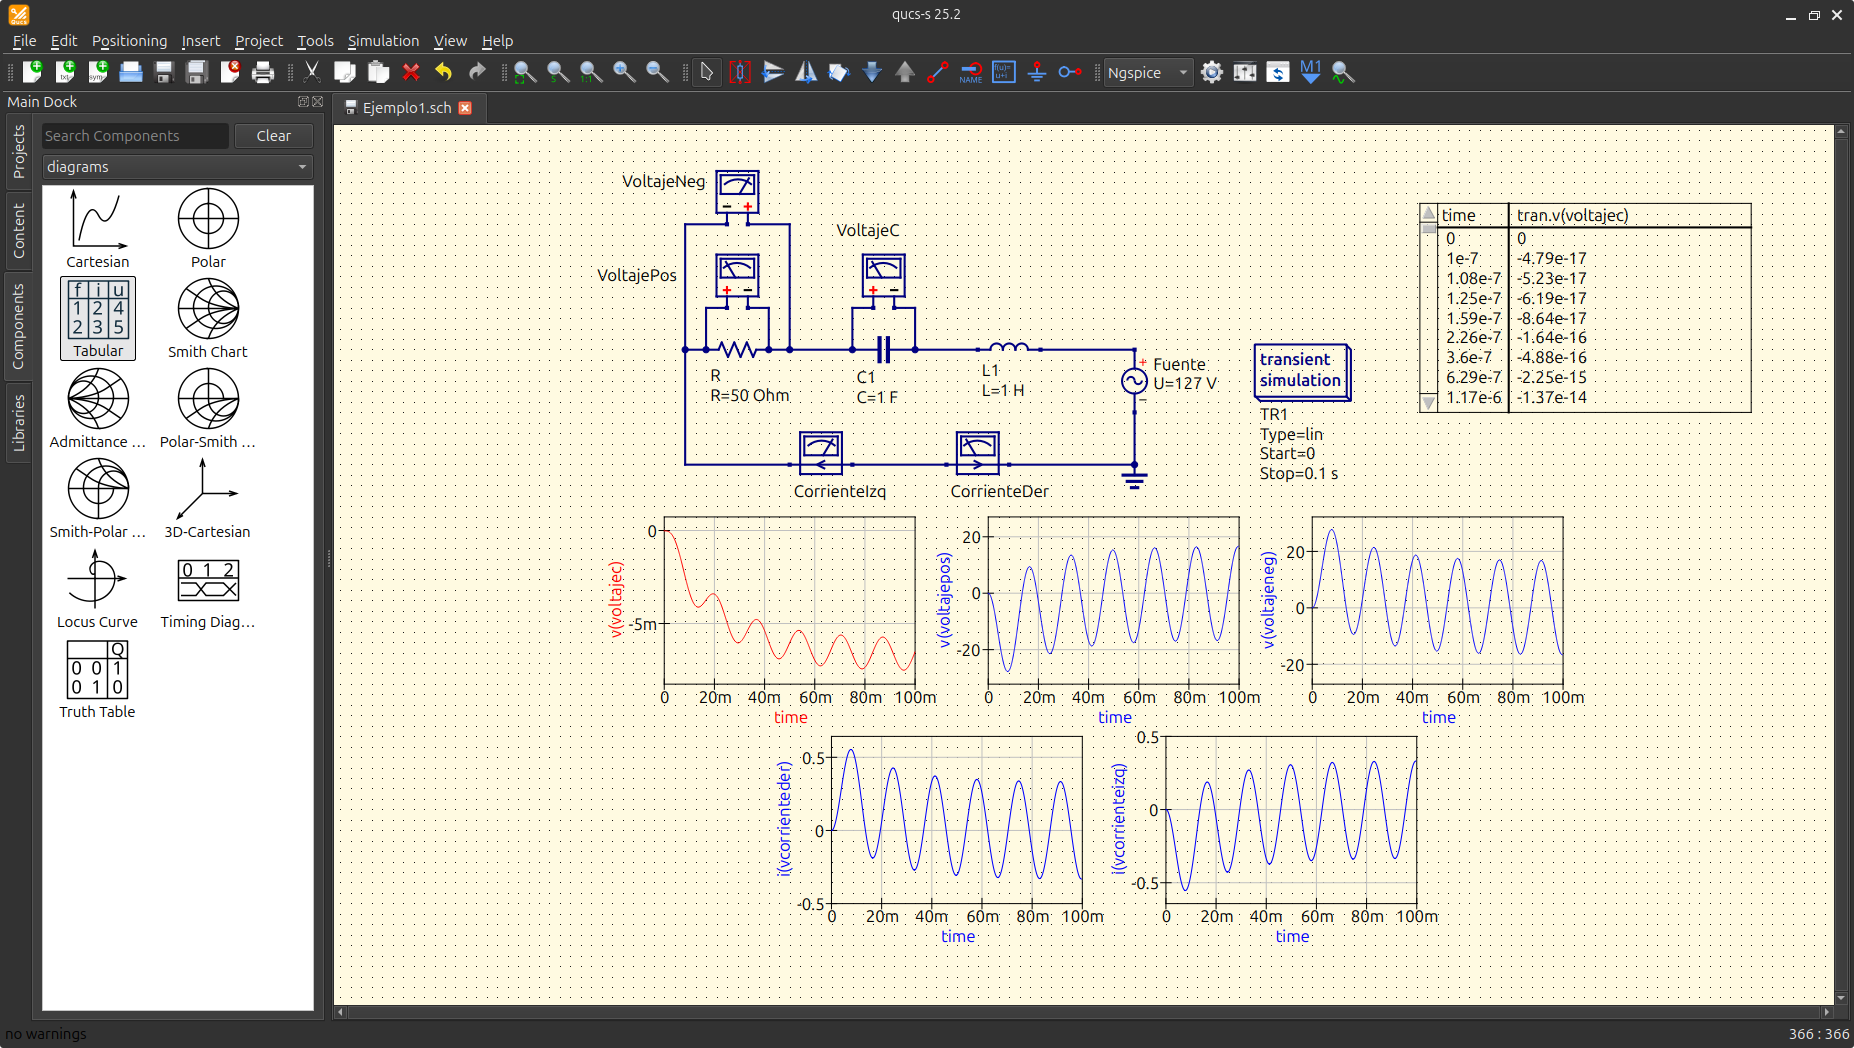
\includegraphics[width=\columnwidth]{Imagenes/Final.png}
    \end{column}
  \end{columns}
\end{frame}

\begin{frame}[fragile]{Librerias}

  \begin{columns}[T]
    % Columna izquierda para el texto
    \begin{column}{0.5\textwidth}
      \begin{enumerate}
        \setcounter{enumi}{3} % Continuar la numeración desde el 4
        \item \textbf{Tipos de Librerias.}
          \begin{itemize}
            \item Existe mucha variedad de bibliotecas incluidas en QUCS-S.
            \item Adicionalmente podemos agregar componentes propios a través de archivos \textit{PSpice Model} proporcionados por los fabricantes.
          \end{itemize}
      \end{enumerate}
    \end{column}

    % Columna derecha para la imagen
    \begin{column}{0.4\textwidth}
      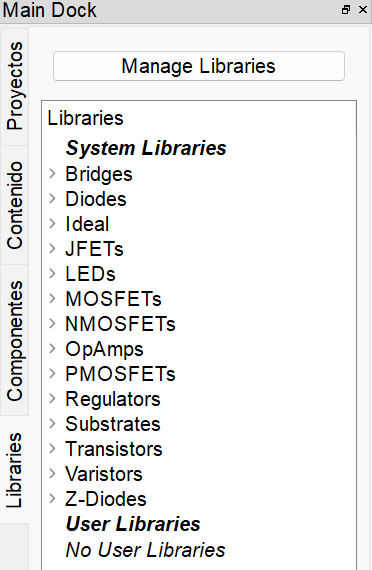
\includegraphics[width=\columnwidth]{Imagenes/Lib.png}
    \end{column}
  \end{columns}
\end{frame}

% --- Diapositiva de Preguntas ---
\begin{frame}
  \begin{center}
    \Huge \textbf{¿Preguntas?}
  \end{center}
\end{frame}

\end{document}